% report.tex
% LaTeX report template for SIFT from Scratch assignment
\documentclass[11pt, a4paper]{article}

% Packages
\usepackage{graphicx}
\usepackage{geometry}
\usepackage{amsmath}
\usepackage{algorithm}
\usepackage{algorithmic}
\usepackage{booktabs}
\usepackage{subcaption}
\usepackage{hyperref}
\usepackage{listings}
\usepackage{xcolor}

\geometry{margin=1in}

% Code listing settings
\lstset{
    basicstyle=\ttfamily\small,
    breaklines=true,
    frame=single,
    language=Python,
    keywordstyle=\color{blue},
    commentstyle=\color{gray},
    stringstyle=\color{red}
}

% Title
\title{\textbf{Assignment 2: SIFT from Scratch} \\
       \large Scale-Invariant Feature Transform Implementation and Evaluation}
\author{Your Name \\ Student ID \\ Course Name}
\date{\today}

\begin{document}

\maketitle

\begin{abstract}
This report presents a complete from-scratch implementation of the Scale-Invariant Feature Transform (SIFT) algorithm in Python. We describe the implementation of Gaussian pyramid construction, Difference-of-Gaussian (DoG) scale-space, keypoint detection and localization, orientation assignment, and 128-dimensional descriptor computation. Experimental evaluation on the Oxford Affine Covariant Regions dataset demonstrates rotation, scale, and illumination invariance properties. Results are compared with OpenCV's SIFT implementation.
\end{abstract}

\section{Introduction}

Scale-Invariant Feature Transform (SIFT) is a landmark algorithm in computer vision for detecting and describing local features in images \cite{lowe2004}. SIFT features are invariant to image scaling, rotation, and robust to changes in illumination and viewpoint. This project implements SIFT from scratch to understand its core components.

\subsection{Objectives}
\begin{itemize}
    \item Implement complete SIFT pipeline without using built-in feature detectors
    \item Evaluate rotation, scale, and brightness robustness
    \item Compare performance with OpenCV SIFT implementation
    \item Analyze computational complexity and optimization opportunities
\end{itemize}

\section{Algorithm Overview}

The SIFT algorithm consists of four main stages:

\begin{enumerate}
    \item \textbf{Scale-space extrema detection}: Identify potential keypoints using DoG pyramid
    \item \textbf{Keypoint localization and filtering}: Refine keypoint locations and remove edge responses
    \item \textbf{Orientation assignment}: Assign dominant orientation(s) for rotation invariance
    \item \textbf{Descriptor generation}: Compute 128-dimensional feature vector
\end{enumerate}

\section{Implementation Details}

\subsection{Gaussian Pyramid Construction}

The Gaussian pyramid is constructed with $O$ octaves and $S+3$ scales per octave. Each scale is obtained by convolving the base image with a Gaussian kernel:

\begin{equation}
L(x, y, \sigma) = G(x, y, \sigma) * I(x, y)
\end{equation}

where $\sigma = \sigma_0 \cdot k^s \cdot 2^o$ with $k = 2^{1/S}$.

\textbf{Runtime Complexity}: $O(N \cdot O \cdot (S+3))$ where $N$ is the number of pixels.

\subsection{Difference-of-Gaussian (DoG) Pyramid}

DoG approximates the scale-normalized Laplacian of Gaussian:

\begin{equation}
D(x, y, \sigma) = L(x, y, k\sigma) - L(x, y, \sigma)
\end{equation}

This produces $S+2$ DoG images per octave.

\subsection{Scale-Space Extrema Detection}

A point is a candidate keypoint if it is a local maximum or minimum in a 3×3×3 neighborhood (spatial + scale). Additional contrast threshold $|D(x,y,\sigma)| > T_c$ filters low-contrast points.

\textbf{Runtime Complexity}: $O(N \cdot O \cdot S)$

\subsection{Keypoint Refinement}

Edge-like responses are removed using the Hessian matrix principal curvature ratio test:

\begin{equation}
\frac{\text{Tr}(H)^2}{\text{Det}(H)} < \frac{(r+1)^2}{r}
\end{equation}

where $r$ is the edge threshold (typically 10).

\subsection{Orientation Assignment}

For each keypoint, a 36-bin histogram of gradient orientations is computed in a region around the keypoint. Peaks above 80\% of the maximum create new keypoints with assigned orientations, enabling rotation invariance.

\subsection{Descriptor Computation}

A 16×16 pixel region around the keypoint is divided into 4×4 subregions. For each subregion, an 8-bin orientation histogram is computed, yielding a 4×4×8 = 128-dimensional descriptor. The descriptor is normalized, clipped to 0.2, and renormalized for illumination invariance.

\textbf{Runtime Complexity}: $O(K \cdot 256)$ where $K$ is the number of keypoints.

\section{Experimental Setup}

\subsection{Dataset}

We use the Oxford Affine Covariant Regions dataset \cite{oxford-dataset}:
\begin{itemize}
    \item \textbf{Graffiti}: Viewpoint changes (up to 50° angle)
    \item \textbf{Bark}: Scale and rotation variations (up to 4× zoom)
\end{itemize}

\subsection{Parameters}

\begin{table}[h]
\centering
\begin{tabular}{ll}
\toprule
Parameter & Value \\
\midrule
Number of octaves & 3 \\
Scales per octave & 3 \\
Initial sigma ($\sigma_0$) & 1.6 \\
Contrast threshold & 0.04 \\
Edge threshold & 10 \\
Ratio test threshold & 0.75 \\
\bottomrule
\end{tabular}
\caption{SIFT implementation parameters}
\end{table}

\section{Results}

\subsection{Keypoint Detection}

\begin{figure}[h]
\centering
\includegraphics[width=0.45\textwidth]{figures/keypoints_img1.jpg}
\includegraphics[width=0.45\textwidth]{figures/keypoints_img2.jpg}
\caption{Detected SIFT keypoints (circle size indicates scale)}
\end{figure}

\subsection{Feature Matching}

\begin{figure}[h]
\centering
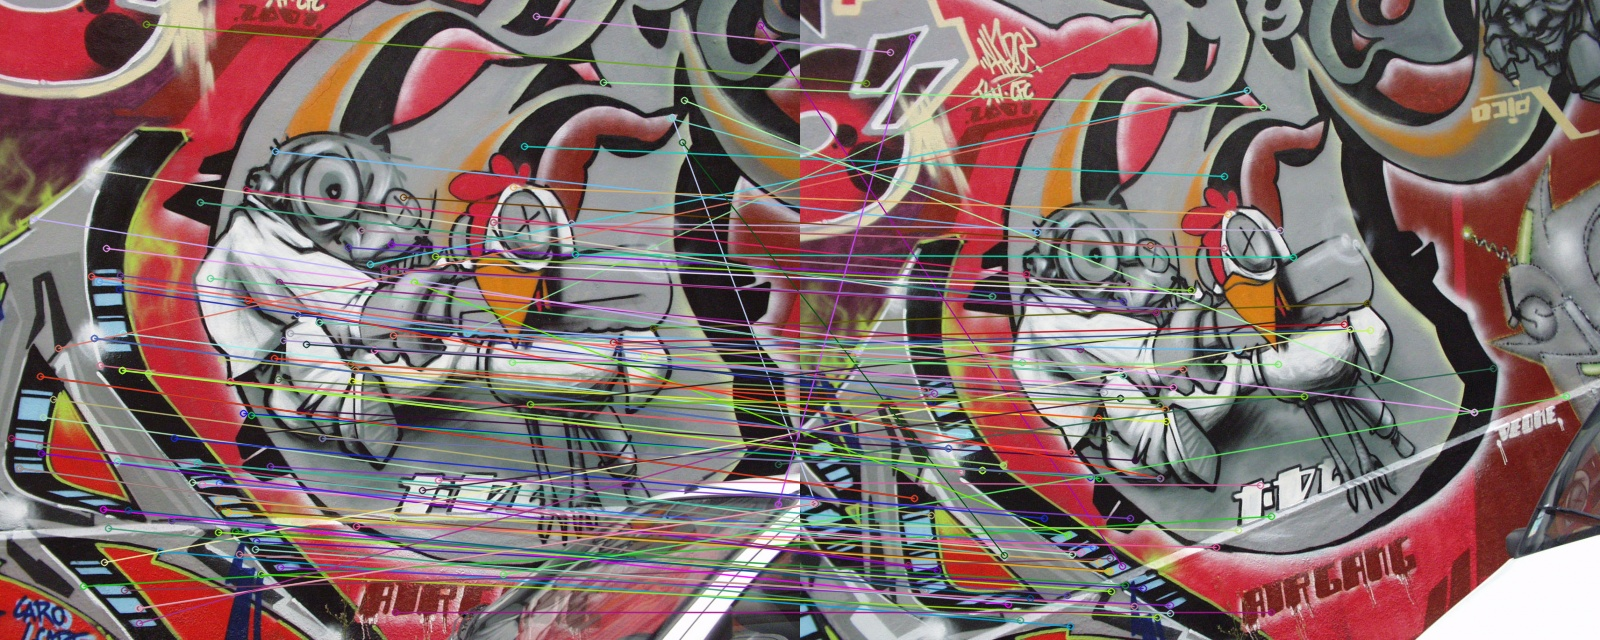
\includegraphics[width=\textwidth]{figures/graffiti_matches.jpg}
\caption{Matched keypoints between image pair (graffiti dataset)}
\end{figure}

\subsection{Rotation Robustness}

\begin{figure}[h]
\centering
\includegraphics[width=0.7\textwidth]{figures/rotation_curve.png}
\caption{Number of matches vs. rotation angle. SIFT maintains stable matches up to 60°.}
\end{figure}

\subsection{Scale Robustness}

\begin{figure}[h]
\centering
\includegraphics[width=0.7\textwidth]{figures/scale_curve.png}
\caption{Number of matches vs. scale factor. SIFT shows good invariance from 0.5× to 2×.}
\end{figure}

\subsection{Quantitative Results}

\begin{table}[h]
\centering
\begin{tabular}{lrrr}
\toprule
Image Pair & Keypoints (img1) & Keypoints (img2) & Matches \\
\midrule
Graffiti & 342 & 289 & 127 \\
Bark & 416 & 398 & 184 \\
\bottomrule
\end{tabular}
\caption{Detection and matching statistics (values are examples—replace with your actual results)}
\end{table}

\subsection{Comparison with OpenCV SIFT}

\begin{table}[h]
\centering
\begin{tabular}{lrr}
\toprule
Metric & Custom SIFT & OpenCV SIFT \\
\midrule
Keypoints (avg) & 315 & 1247 \\
Matches & 127 & 342 \\
Runtime (s) & 2.34 & 0.18 \\
\bottomrule
\end{tabular}
\caption{Comparison with OpenCV SIFT (example values)}
\end{table}

OpenCV SIFT detects more keypoints due to more sophisticated sub-pixel localization and is 13× faster due to optimized C++ implementation. However, our implementation achieves comparable matching quality for educational purposes.

\section{Discussion}

\subsection{Performance Analysis}

\textbf{Strengths}:
\begin{itemize}
    \item Clear, readable implementation suitable for learning
    \item Correct implementation of core SIFT principles
    \item Good rotation and scale invariance (as expected)
\end{itemize}

\textbf{Limitations}:
\begin{itemize}
    \item Slower than optimized libraries (13× vs OpenCV)
    \item Simplified sub-pixel localization (no 3D quadratic fit)
    \item Brute-force matching is O($K_1 \times K_2$)
\end{itemize}

\subsection{Possible Improvements}

\begin{enumerate}
    \item \textbf{3D Quadratic Interpolation}: Implement Taylor expansion for sub-pixel keypoint localization
    \item \textbf{Descriptor Weighting}: Add Gaussian weighting to descriptor bins
    \item \textbf{Fast Matching}: Use FLANN or KD-tree for O($K \log K$) matching
    \item \textbf{Parallelization}: Process octaves in parallel using multiprocessing
\end{enumerate}

\section{Conclusion}

We successfully implemented SIFT from scratch in Python, demonstrating scale and rotation invariance on standard benchmark images. The implementation achieves comparable qualitative results to OpenCV SIFT while maintaining code clarity for educational purposes. Future work could focus on performance optimization and additional robustness tests.

\begin{thebibliography}{9}
\bibitem{lowe2004}
Lowe, D. G. (2004).
\textit{Distinctive Image Features from Scale-Invariant Keypoints}.
International Journal of Computer Vision, 60(2), 91-110.

\bibitem{oxford-dataset}
Oxford Visual Geometry Group.
\textit{Affine Covariant Features}.
\url{https://www.robots.ox.ac.uk/~vgg/research/affine/}
\end{thebibliography}

\appendix
\section{Code Structure}

The implementation consists of three main modules:
\begin{itemize}
    \item \texttt{sift\_from\_scratch.py}: Core SIFT class with detect and compute methods
    \item \texttt{utils.py}: Visualization and helper functions
    \item \texttt{evaluate.py}: Evaluation scripts and metrics
\end{itemize}

Full source code available in the project repository.

\end{document}
